% Options for packages loaded elsewhere
\PassOptionsToPackage{unicode}{hyperref}
\PassOptionsToPackage{hyphens}{url}
\PassOptionsToPackage{dvipsnames,svgnames,x11names}{xcolor}
\documentclass[
  12pt,
  letterpaper,
]{article}
\usepackage{xcolor}
\usepackage[margin=1in]{geometry}
\usepackage{amsmath,amssymb}
\setcounter{secnumdepth}{-\maxdimen} % remove section numbering
\usepackage{iftex}
\ifPDFTeX
  \usepackage[T1]{fontenc}
  \usepackage[utf8]{inputenc}
  \usepackage{textcomp} % provide euro and other symbols
\else % if luatex or xetex
  \usepackage{unicode-math} % this also loads fontspec
  \defaultfontfeatures{Scale=MatchLowercase}
  \defaultfontfeatures[\rmfamily]{Ligatures=TeX,Scale=1}
\fi
\usepackage[]{newtxtext,newtxmath}
\ifPDFTeX\else
  % xetex/luatex font selection
\fi
% Use upquote if available, for straight quotes in verbatim environments
\IfFileExists{upquote.sty}{\usepackage{upquote}}{}
\IfFileExists{microtype.sty}{% use microtype if available
  \usepackage[]{microtype}
  \UseMicrotypeSet[protrusion]{basicmath} % disable protrusion for tt fonts
}{}
\makeatletter
\@ifundefined{KOMAClassName}{% if non-KOMA class
  \IfFileExists{parskip.sty}{%
    \usepackage{parskip}
  }{% else
    \setlength{\parindent}{0pt}
    \setlength{\parskip}{6pt plus 2pt minus 1pt}}
}{% if KOMA class
  \KOMAoptions{parskip=half}}
\makeatother
\usepackage{longtable,booktabs,array}
\newcounter{none} % for unnumbered tables
\usepackage{calc} % for calculating minipage widths
% Correct order of tables after \paragraph or \subparagraph
\usepackage{etoolbox}
\makeatletter
\patchcmd\longtable{\par}{\if@noskipsec\mbox{}\fi\par}{}{}
\makeatother
% Allow footnotes in longtable head/foot
\IfFileExists{footnotehyper.sty}{\usepackage{footnotehyper}}{\usepackage{footnote}}
\makesavenoteenv{longtable}
\usepackage{graphicx}
\makeatletter
\newsavebox\pandoc@box
\newcommand*\pandocbounded[1]{% scales image to fit in text height/width
  \sbox\pandoc@box{#1}%
  \Gscale@div\@tempa{\textheight}{\dimexpr\ht\pandoc@box+\dp\pandoc@box\relax}%
  \Gscale@div\@tempb{\linewidth}{\wd\pandoc@box}%
  \ifdim\@tempb\p@<\@tempa\p@\let\@tempa\@tempb\fi% select the smaller of both
  \ifdim\@tempa\p@<\p@\scalebox{\@tempa}{\usebox\pandoc@box}%
  \else\usebox{\pandoc@box}%
  \fi%
}
% Set default figure placement to htbp
\def\fps@figure{htbp}
\makeatother
\setlength{\emergencystretch}{3em} % prevent overfull lines
\providecommand{\tightlist}{%
  \setlength{\itemsep}{0pt}\setlength{\parskip}{0pt}}
\usepackage{caption}\captionsetup[figure]{labelformat=empty}
\usepackage{bookmark}
\IfFileExists{xurl.sty}{\usepackage{xurl}}{} % add URL line breaks if available
\urlstyle{same}
\hypersetup{
  pdftitle={How Much Incorrect Retrieved Context Does It Take to Flip an LLM\textquotesingle s Answer?},
  pdfauthor={Zane Braunstein and Donovan Sappet},
  colorlinks=true,
  linkcolor={black},
  filecolor={Maroon},
  citecolor={Blue},
  urlcolor={black},
  pdfcreator={LaTeX via pandoc}}

\title{How Much Incorrect Retrieved Context Does
It Take to Flip an LLM\textquotesingle s Answer?}
\usepackage{etoolbox}
\makeatletter
\providecommand{\subtitle}[1]{% add subtitle to \maketitle
  \apptocmd{\@title}{\par {\large #1 \par}}{}{}
}
\makeatother
\subtitle{COMP 345 Midterm Report}
\author{Zane Braunstein and Donovan Sappet}
\date{October 30, 2026}

\begin{document}
\maketitle

\section{1. Problem}\label{problem}

People increasingly turn to AI chatbots for news.
In 2026, 10\% of people surveyed across 48
countries and territories used an AI chatbot such
as ChatGPT, Perplexity, or Google Gemini for news
each week, up from 7\% a year earlier (Egan et
al.~2026). Many of these chatbots look up
documents and read them before answering a
question, a design known as retrieval-augmented
generation (RAG; Lewis et al.~2020). When the
question is about news or policy, the documents a
chatbot finds may be out of date or wrong. If
those documents contain wrong information, the
model may repeat that wrong information even when
it already knows the correct answer. As this use
continues to grow, it becomes more important to
understand how incorrect facts in these documents
affect the model's answers.

This project is a stress test of how a
retrieval-augmented LLM handles incorrect
information in the documents it collects. We
measure how much incorrect context an LLM needs to
see before its answer flips to the wrong value,
and we test whether the model's hidden states can
predict when the flip occurs.

\subsection{1.1 Our Approach}\label{our-approach}

We study a RAG system in which an open-weight LLM,
Llama 3.1 8B Instruct, answers a question after
reading passages of related text. Our text comes
from 2,047 research publications by Rice
University's Baker Institute for Public Policy and
the 747 PDF reports those publications link to,
split into short passages. For each question we
test, we choose 5 passages that state the correct
answer. A retriever (all-MiniLM-L6-v2) scores how
closely each passage matches the question and puts
the 5 passages in order, from most to least
similar. The ordered passages are then pasted
ahead of the question into Llama's prompt.

To test how wrong context changes the answer, we
edit \(m\) of the 5 passages to state a wrong
(counterfactual) value, for \(m = 0\) to 5,
choosing which passages to edit from a random
order (Section 6.3). A script then checks whether
Llama's answer states the true value, the wrong
value, both, or neither. We test Llama's
performance under three conditions, which differ
only in the passages placed in the prompt.
Condition 1 asks the question with no passages, to
find out whether Llama already knows the answer.
Condition 2 provides the 5 unedited passages.
Condition 3 edits 1 to 5 of those passages. For
every prompt, we also save Llama's hidden states
(the internal vectors the model computes at each
of its 32 layers) and train simple
classifiers---hereafter called probes---to predict
from these vectors whether Llama's answer will
state the true value.

In our midterm sample of 20 facts, Llama's answers
flip in more than half of cases once 2 of the 5
passages are edited, stating the wrong value
either alone or alongside the true value. This
happens whether or not the model knew the fact
beforehand. Which passage is edited also matters:
an edit to the first passage lowers the share of
correct answers more than four times as much as an
edit to the last passage. A first set of probes,
trained on 16 facts, does not yet predict the flip
on facts outside its training set, but we expect
the probes to improve once they are trained on the
full set of about 100 facts (Section 7.6).

\textbf{{[}TODO: Figure 1, the simple pipeline
figure Shrish asked for: question + 5 passages →
retriever orders them → edit m of them → Llama →
answer and hidden states → scoring script and
probes.{]}}

\emph{Figure 1: Overview of one example, from the
question and its 5 passages to the scored answer
and the saved hidden states.}

\section{2. Hypothesis}\label{hypothesis}

We test Llama on facts split into two groups:
\emph{parametric} facts are those the model
learned during pretraining and stores in its
weights, and \emph{extractive} facts are those the
model has never seen, which it can learn only from
the retrieved passages (Section 4.2). For each
question, we give the model 5 passages that each
state the correct answer and edit \(m\) of them to
state a wrong (counterfactual) value. For each
prompt, we collect one greedy answer, which always
takes the most likely next word, and 10 sampled
answers, which choose each next word at random
according to the model's probabilities. We measure
the model's response as the true-answer rate---the
fraction of its sampled answers that state the
true value (Section 6.6). Because the true-answer
rate is built from 10 sampled answers, it shows
how confident the model is in the true value, not
only which answer it gives most often.

We conjecture three key relationships between the
model results and the input data:

\begin{enumerate}
\def\labelenumi{\arabic{enumi}.}
\tightlist
\item
  As \(m\) increases, the model's answers shift
  (flip) from the true value to the counterfactual
  one. We expect that for most facts the
  true-answer rate drops sharply over one or two
  values of \(m\) rather than declining steadily.
\item
  We expect extractive facts to flip at a lower
  \(m\) than parametric facts, since the model has
  no stored answer to compare the passages
  against.
\item
  We posit that a linear probe trained on the
  model's hidden states can predict whether the
  model will side with its pretrained knowledge or
  the retrieved context, even among examples with
  the same \(m\), where a classifier given only
  \(m\) cannot tell them apart. We expect this
  information to be strongest in the middle
  layers, consistent with Zhao et al.~(2024).
\end{enumerate}

\section{3. Related
Approaches}\label{related-approaches}

It is well established that retrieval improves LLM
accuracy and that irrelevant context can make
answers worse (Shi et al.~2023; Liu et al.~2023;
Cuconasu et al.~2024). Previous studies reach
conflicting conclusions about how a model behaves
when retrieved context directly contradicts what
the model learned in pretraining. Longpre et
al.~(2021) found that QA models over-rely on
memorized knowledge and ignore context that
contradicts their memory. Xie et al.~(2024) found
the opposite for newer LLMs, which readily accept
contradicting evidence when it is coherent, but
still favor evidence that agrees with their memory
when both are present. Wu et al.~(2024, ClashEval)
found that LLMs adopt incorrect retrieved content
over their own correct prior knowledge over 60\%
of the time, and are more likely to do so when
they are less confident in the prior answer.

Most of these studies measure only the model's
outputs. Zhao et al.~(2024) extended this work by
studying the model's internal states when it is
given conflicting context. The researchers trained
logistic-regression probes on the hidden states
(the residual stream) of Llama 3 8B and found that
these hidden states signal a conflict between
context and memory in the middle layers, peaking
around layer 14 of 32. Zhao et al.'s probes could
also predict, before the answer was generated,
whether Llama would answer from the context or
from its memory. However, their setup gives the
model a single conflicting passage rather than
varying how much of the context conflicts. It also
compares that passage against the model's own
closed-book answer, so it does not separate facts
the model knows from facts it does not.

Building on this research regarding how LLMs
handle conflicts between retrieved context and
their memory, and in particular on Zhao et
al.~(2024), we vary the amount of conflicting
context as a controlled dose (\(m = 0\) to 5 of 5
passages) rather than using one conflict
condition. We place the edited passages inside a
full retrieval pipeline over real policy
documents, rather than giving the model one
prepared passage from a standard QA benchmark, so
the text is written for real readers rather than
built for testing. We compare facts the model
knows (parametric) with facts it does not
(extractive). We also test whether the probe can
tell apart examples with the same number of wrong
passages, for example two facts at \(m = 3\) where
Llama keeps one and flips the other. A classifier
given only \(m\) cannot do this, so a probe with
this ability would show that the hidden states
carry information about the model's choice beyond
the input it was given.

Our initial results partly agree with Liu et
al.~(2023), who found that language models make
the best use of information placed at the start or
end of a long input, and the worst use of
information in the middle. In our experiment,
editing the first of the 5 passages lowers the
share of correct answers far more than editing any
other passage, but editing either of the last two
passages has the smallest effect (Section 7.5). In
other words, we observe a primacy effect (the
first passage carries the most weight) but no
recency effect (the last passages carry the
least). In our setup, the first passage is also
the passage most similar to the question, so part
of this effect may come from how closely the
passage matches the question rather than from its
position.

\section{4. Datasets}\label{datasets}

\subsection{4.1 Corpus}\label{corpus}

Our corpus is the research published by Rice
University's Baker Institute for Public Policy. A
web scraper collected every research page on the
Baker Institute website, along with the text of
the PDF reports those pages link to. The scraper
takes its list of pages from the site's public
sitemap and sends one request per second. The
site's \texttt{robots.txt} file, which tells
automated crawlers which parts of the site they
may visit, disallows a separate
\texttt{/research-library} section, so we did not
collect that section.

The sitemap lists 4,271 pages. Of these, 2,054 are
research publications; most of the rest are event
pages (1,765) and expert and staff profiles (252).
Our scraper collected 2,047 of the research pages,
published between 2016 and 2026 (791 of them in
2024 or later), along with 747 PDF reports linked
from 717 of those pages. A research page is often
a summary of the full report, which is linked as a
PDF: the median page has 855 words, while the
median PDF has 3,890. In total, the pages hold 3.3
million words and the PDFs hold 4.4 million.

A single report can be thousands of words long and
cover many topics, so the retriever and our search
tools work with short passages rather than whole
documents. Each document is split into passages of
at least 120 words, so that each passage is long
enough to state a fact along with its surrounding
context, which is what we look for when choosing
the 5 passages for each question (Section 4.3). To
keep each passage's context intact, each passage
is built from full paragraphs, so a paragraph is
never cut in half. As a result, most passages run
a little over 120 words (median 139; Figure 2).
The corpus has 50,852 passages. Of these, 87\% are
between 120 and 200 words, 10\% are longer
(usually one long paragraph or a table), and 4\%
are shorter (the last passage of a document, when
fewer than 120 words are left).

All of these passages stay in the corpus,
including the short and the long ones. Only the
passages we choose for a fact (Section 4.3) have
an upper limit of 200 words. The retriever reads
only the first 256 tokens of a passage (about 200
words) and ignores the rest, so a passage of at
most 200 words lets the retriever's score cover
the whole passage, including the sentence that
states the fact. Of the 310 passages chosen for
our 62 facts, 8 are longer (up to 288 words),
because those facts had no shorter passage to use
in their place. The 200-word limit matters only
for the retriever. Llama reads every passage in
full, so a longer passage can only change the
order in which the retriever places the 5
passages, and Section 7.5 shows that this order
matters.

A research page often repeats sentences from its
own PDF (for example, its executive summary), so
the same sentence can appear in two passages of
the corpus. Section 4.3 explains how we handle
these copies when choosing a fact's passages.

\begin{figure}
\centering
\pandocbounded{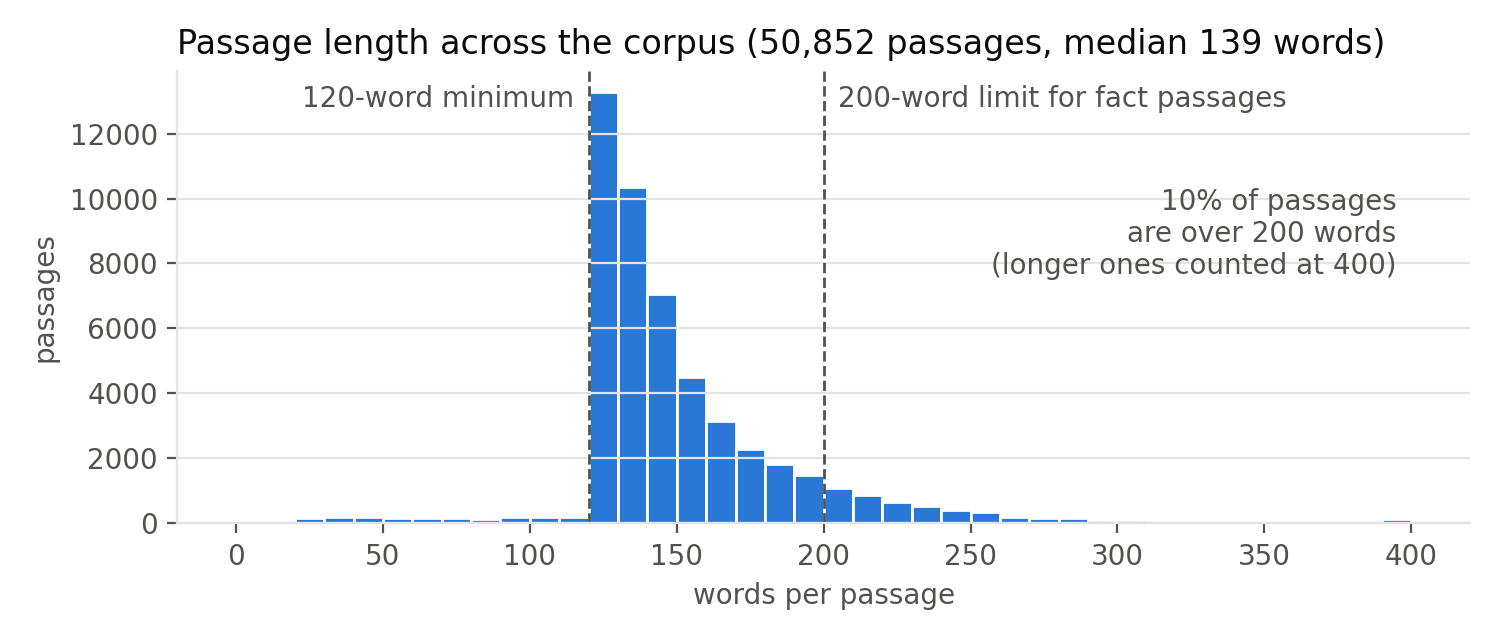
\includegraphics[keepaspectratio,alt={Figure 2: Passage length across the corpus. Passages over 400 words are counted at 400.}]{figures/comp345-midterm-fig-passage-lengths.png}}
\caption{Figure 2: Passage length across the
corpus. Passages over 400 words are counted at
400.}
\end{figure}

\subsection{4.2 Facts}\label{facts}

A fact in our study is a number, name, or date
that answers a short question, such as the year
NAFTA went into effect (1994). We use short
answers for two reasons: each fact has one clear
value, which is easy to replace with a single
wrong value, and a script can check which of the
two values the model's answer states. Each fact
has 3 differently worded versions of its question,
so that a result does not depend on one phrasing
(Section 6.3). We aim for about 100 facts in the
final report. At the time of this report, 62 have
been checked by hand, and this report tests a
sample of 20 (Section 4.4).

Our second hypothesis (Section 2) compares how
easily two kinds of facts flip, so each fact is
assigned to one of the two groups below. Condition
1 (Section 6.1) decides the group by asking each
question with no passages.

\begin{itemize}
\tightlist
\item
  \emph{Parametric} facts are already known to the
  model from pretraining. We count a fact as
  parametric if the model answers all 3 wordings
  correctly with no passages. When an edited
  passage states a different value than the one
  the model learned, the model has to choose
  between its memory and its context.
\item
  \emph{Extractive} facts appear only in the
  corpus, so the model cannot answer these
  questions without the passages. We count a fact
  as extractive if the model does not answer any
  of the 3 wordings correctly with no passages. We
  prefer values from publications after Llama's
  December 2023 training cutoff, which the model
  could not have seen during pretraining. Since
  the model has no stored answer to fall back on,
  these questions show how easily the model
  accepts wrong context when it has nothing to
  compare against.
\end{itemize}

A fact answered correctly for only one or two
wordings fits neither group. We report these
\emph{mixed} facts separately (2 of the 20 facts
in this report; Section 7.1).

For each fact, we wrote one plausible
counterfactual value, close to the true value but
wrong, such as 1996 instead of 1994 for NAFTA. We
avoid obviously false values (such as 1776)
because the model could reject such a value on its
own, without weighing the edited passages against
the unedited ones. A plausible value makes the
model choose between two believable sources, as an
outdated figure or a real error in a document
would. For each fact, every edited passage states
the same counterfactual value. This keeps the
wrong passages in agreement with each other, and
it lets one script pattern recognize the wrong
answer. The number of edited passages, \(m\), then
measures how much support the wrong answer has.
For instance, at \(m = 3\) the model sees three
passages that say NAFTA took effect in 1996 and
two that say 1994.

Because we choose every counterfactual value
ourselves, each question has a known correct
answer. The true value is whatever the unedited
passages say, and the counterfactual value is the
one we inserted. A script checks which of the two
values the model's answer states (Section 6.5), so
scoring needs no human answer key and no LLM
judge. Only answers that state both values, or
neither value, are read and labelled by hand.

\subsection{4.3 Passages for Each
Fact}\label{passages-for-each-fact}

Each fact is paired with 5 corpus passages that
state its true value. We choose these passages
ourselves rather than letting the retriever search
the corpus for them, so that we control exactly
how many edited passages the model sees. If the
retriever searched the whole corpus, it would
decide how many of the edited passages reach the
model, and \(m\) would no longer be set by us
(this setting is Condition 4, Section 6.4). With 5
passages per fact, the number of passages carrying
the wrong value can be raised one step at a time
from 0 to 5. This lets us measure the point at
which the incorrect data starts to control the
model's answer, rather than only testing whether a
single wrong passage changes the answer, as in
Zhao et al.~(2024).

The 5 passages must state the fact in 5
non-identical sentences, so that each passage is a
separate statement of the fact rather than a
repeat of another passage. Two passages can come
from the same document, as long as the sentence
stating the fact is worded differently in each.
Most copies come from web pages that paste
sentences from their own PDF reports. To find
them, we compare the sentences that state the
fact. If 90\% of the words in the shorter sentence
appear in the other sentence, in the same order,
the two passages count as copies, and only one of
them can be among the fact's 5 passages. Our
initial rule required the fact to appear in 5
different documents, but fewer Baker documents
cover recent events, so that rule left very few
extractive facts. Each chosen passage should also
be at most 200 words (Section 4.1).

\subsection{4.4 Finding Facts and the Midterm
Sample}\label{finding-facts-and-the-midterm-sample}

We found candidate facts for this report with
three tools:

\begin{itemize}
\tightlist
\item
  A mining script finds subjects and values that
  sit close together in a sentence (for example,
  ``NAFTA'' and ``1994'') and ranks the pairs by
  how many non-identical passages state them. Many
  values appear near a subject only because the
  value is common everywhere (for example,
  ``2024'' near ``Mexico''), so the script keeps a
  pair only if the value appears near the subject
  at least 3 times as often as the value appears
  in the corpus overall.
\item
  A search script lists every passage that matches
  a given pattern. We used this script to choose
  each fact's 5 passages.
\item
  An AI assistant (Claude) used these scripts to
  draft 95 candidate facts with their passages, of
  which we kept 51 after reading every passage.
\end{itemize}

As of this report, we have a total of 62 facts.
Before a fact was used, we read its passages and
confirmed both values, and a script checked that
each edit changes every passage and that the
counterfactual value does not already appear in
the unedited passages.

Condition 1 (Section 6.1) assigns each fact to a
group by asking Llama the question with no
passages. To choose a sample for this report, we
first ran Condition 1 on all 62 facts on a laptop
CPU, using only the greedy answer. Llama answered
all 3 wordings correctly for 43 facts, one or two
wordings correctly for 10, and no wording
correctly for the other 9. We chose 10 parametric
facts that cover different kinds of values (years,
months, percentages, dollar amounts) and 10
extractive facts: the 9 that Llama never answered
correctly, and one (the 2025 tariff on Mexico and
Canada) whose only correct-looking answer quoted
an older tariff. The experiment then repeats
Condition 1 on a Google Colab L4 GPU (Section
5.1), and the greedy answers from that run set
each fact's final group. In that run, all 10
parametric facts were again answered correctly for
every wording, and 8 of the extractive facts were
not answered correctly for any wording. The other
2 (the date of the Hamas attack and the 2025
tariff on Mexico and Canada) were answered
correctly for one wording each, so we report them
as mixed facts (Section 7.1).

\emph{Table 1: The 20 facts in the midterm sample.
``Screen'' is the number of question wordings (of
3) Llama answered correctly with no passages in
the laptop screen used to pick the sample; ``Run''
is the same count in the GPU run, which sets the
final group.}

{\def\LTcaptype{none} % do not increment counter
\begin{longtable}[]{@{}
  >{\raggedright\arraybackslash}p{(\linewidth - 12\tabcolsep) * \real{0.1327}}
  >{\raggedright\arraybackslash}p{(\linewidth - 12\tabcolsep) * \real{0.2449}}
  >{\raggedright\arraybackslash}p{(\linewidth - 12\tabcolsep) * \real{0.1837}}
  >{\raggedright\arraybackslash}p{(\linewidth - 12\tabcolsep) * \real{0.1633}}
  >{\raggedright\arraybackslash}p{(\linewidth - 12\tabcolsep) * \real{0.0816}}
  >{\raggedright\arraybackslash}p{(\linewidth - 12\tabcolsep) * \real{0.0612}}
  >{\raggedright\arraybackslash}p{(\linewidth - 12\tabcolsep) * \real{0.1327}}@{}}
\toprule\noalign{}
\begin{minipage}[b]{\linewidth}\raggedright
Picked as
\end{minipage} &
\begin{minipage}[b]{\linewidth}\raggedright
Fact
\end{minipage} &
\begin{minipage}[b]{\linewidth}\raggedright
True value
\end{minipage} &
\begin{minipage}[b]{\linewidth}\raggedright
Counterfactual
\end{minipage} &
\begin{minipage}[b]{\linewidth}\raggedright
Screen
\end{minipage} &
\begin{minipage}[b]{\linewidth}\raggedright
Run
\end{minipage} &
\begin{minipage}[b]{\linewidth}\raggedright
Final group
\end{minipage} \\
\midrule\noalign{}
\endhead
\bottomrule\noalign{}
\endlastfoot
Parametric & Year NAFTA went into effect & 1994 &
1996 & 3 & 3 & Parametric \\
Parametric & Date the USMCA entered into force &
July 1, 2020 & July 1, 2021 & 3 & 3 &
Parametric \\
Parametric & Year of the U.S.-Mexico Water Treaty
& 1944 & 1948 & 3 & 3 & Parametric \\
Parametric & Month Winter Storm Uri hit Texas &
February 2021 & January 2021 & 3 & 3 &
Parametric \\
Parametric & Year of Mexico's energy reform & 2013
& 2016 & 3 & 3 & Parametric \\
Parametric & Month of Russia's full-scale invasion
of Ukraine & February 2022 & March 2022 & 3 & 3 &
Parametric \\
Parametric & THC limit for hemp under U.S. law &
0.3\% & 0.5\% & 3 & 3 & Parametric \\
Parametric & 2017 tax law's cap on the SALT
deduction & \$10,000 & \$15,000 & 3 & 3 &
Parametric \\
Parametric & 2017 tax law's corporate tax rate &
21\% & 23\% & 3 & 3 & Parametric \\
Parametric & Year Hurricane Harvey flooded Houston
& 2017 & 2018 & 3 & 3 & Parametric \\
Extractive & Start of the U.S.-Israeli strikes on
Iran & February 28, 2026 & March 7, 2026 & 0 & 0 &
Extractive \\
Extractive & President of Mexico from October 2024
& Claudia Sheinbaum & Xóchitl Gálvez & 0 & 0 &
Extractive \\
Extractive & Date of the 2023 Hamas attack on
Israel & October 7, 2023 & October 14, 2023 & 0 &
1 & Mixed \\
Extractive & Secretary of State in the second
Trump administration & Marco Rubio & Bill Hagerty
& 0 & 0 & Extractive \\
Extractive & Prime minister of Canada from 2025 &
Mark Carney & Chrystia Freeland & 0 & 0 &
Extractive \\
Extractive & Year Mexico became the top U.S.
trading partner & 2023 & 2021 & 0 & 0 &
Extractive \\
Extractive & Director of the Baker Institute &
David M. Satterfield & Ryan C. Crocker & 0 & 0 &
Extractive \\
Extractive & 2025 U.S. tariff on steel, aluminum,
and copper & 50\% & 40\% & 0 & 0 & Extractive \\
Extractive & 2025 U.S. tariff on Mexico and Canada
(fentanyl and migration) & 25\% & 15\% & 1 & 1 &
Mixed \\
Extractive & Month Claudia Sheinbaum took office &
October 2024 & December 2024 & 0 & 0 &
Extractive \\
\end{longtable}
}

\section{5. Models and
Workflow}\label{models-and-workflow}

\subsection{5.1 Pipeline}\label{pipeline}

The system has three parts (Figure 3):

\begin{itemize}
\tightlist
\item
  The retriever, all-MiniLM-L6-v2, is a pretrained
  sentence-embedding model. It converts the
  question and each passage into a 384-dimensional
  vector and scores each passage by the cosine
  similarity between its vector and the question's
  vector. In Conditions 2 and 3, the retriever
  does not search the whole corpus. Instead, it
  orders each fact's 5 chosen passages, from most
  similar (Passage 1) to least similar (Passage
  5), for the reason given in Section 4.3. The
  retriever is pretrained, and we do not train it
  further.
\item
  The generator, Llama 3.1 8B Instruct, is an
  open-weight LLM with a training cutoff of
  December 2023. The ordered passages are pasted
  into a fixed prompt template ahead of the
  question, so Llama reads the passages as plain
  text. We ran Llama on a laptop CPU during
  development and run the experiments on a Google
  Colab L4 GPU.
\item
  The probes are logistic regression classifiers
  trained on Llama's hidden states (Section 5.4).
\end{itemize}

We use a small open-weight model for two reasons:
a small model is likely easier to mislead with
wrong context than the largest commercial LLMs,
and the probes need direct access to the hidden
states, which services offered only through an
online API do not provide. If time permits, we
will repeat the experiment with Llama 3.2 3B to
see whether model size changes the flip point.

\textbf{{[}Figure 3 from the proposal: Canva
design DAHWOkhmehU, page 3. TODO: if its arrows
say the question ``retrieves'' the passages,
change them to show the retriever ordering the
fact's 5 passages.{]}}

\emph{Figure 3: Data flow for one example. The
retriever orders the fact's 5 passages, and m of
them are edited before they reach the frozen LLM.
The generated answer is scored into a truth label,
which is also the training target for the linear
probes on the LLM's hidden states. The 10 sampled
answers per prompt give the true-answer rate.}

\subsection{5.2 Input}\label{input}

Each prompt contains a natural-language question
about one fact and the \(k = 5\) passages that
state the correct answer, in the order the
retriever gives them, with \(m\) of the passages
edited to state the counterfactual value (Section
6.3 explains which passages are edited). Each
combination of fact, question wording, and \(m\)
is one example, so 100 facts, 3 wordings, and 6
values of \(m\) (0 to 5) give 1,800 examples in
the full experiment. The midterm run uses the 20
facts in Table 1, which gives 360 examples, plus
60 closed-book prompts for Condition 1.

\subsection{5.3 Output}\label{output}

For every prompt, the pipeline saves four outputs.
The answers and their labels give the
truth-support rate and the true-answer rate
(Section 6.6), and the hidden states, paired with
the greedy answer's label, train the probes
(Section 6.7):

\begin{itemize}
\tightlist
\item
  Llama's greedy answer, in natural language.
\item
  The scoring script's label for that answer:
  true, counterfactual, both, or neither. The
  probes use a binary version of this label (1 for
  true, 0 otherwise).
\item
  10 sampled answers, each labelled by the same
  script, which give the true-answer rate.
\item
  Llama's hidden states for the prompt. Each of
  Llama's 32 layers produces a 4096-dimensional
  vector for every prompt token. Llama reads text
  from left to right, so each token's vector
  depends only on the tokens before that token.
  The final prompt token is therefore the only one
  that has seen the full question and all 5
  passages, and we save its vector from each layer
  (one 32 × 4096 table of numbers per example).
\end{itemize}

\subsection{5.4 Model Class}\label{model-class}

The pipeline uses three kinds of model, and only
the third is trained by us:

\begin{itemize}
\tightlist
\item
  Embedding model: all-MiniLM-L6-v2 (pretrained,
  frozen), which orders the passages.
\item
  LLM: Llama 3.1 8B Instruct (pretrained, frozen),
  which generates the answer.
\item
  Linear probes: logistic regression with no
  hidden layers. Each probe takes one layer's
  4096-dimensional hidden-state vector \(h\) from
  an example and outputs
  \(p = \sigma(w \cdot h + b)\), where \(\sigma\)
  is the sigmoid function and \(p\) is the
  predicted probability that the LLM's answer for
  that example states the true value. Each probe
  has 4096 weights \(w\) plus 1 bias \(b\) (4097
  parameters). We train one separate probe per
  layer (32 probes) and evaluate each probe on its
  own, so the output is a test accuracy for every
  layer. We do not combine the layers into one
  large probe, because that would hide which layer
  carries the information. With over 130,000
  inputs and only about 1,400 training examples,
  one large probe would also overfit, fitting
  noise in the training examples that does not
  carry over to new facts.
\end{itemize}

The embedding model and LLM are not fine-tuned,
and the prompt template (``Use the passages below
to answer the question. Passage 1: \ldots{}
Passage 5: \ldots{} Question: \ldots{} Answer:'')
is the same in every condition, so any change in
the answer comes from the passages or from the
question wording (Section 4.2). The only learned
parameters are the probe weights.

Because Llama 3.1 Instruct is a chat model, we
send the filled-in template as a single message
from the user. Llama's chat format also adds a
short system message with the current date
(``Today Date: \ldots{}''). The default date, 26
July 2024, made Llama describe 2026 events as
hypothetical, so we fix the date to 26 October
2026 in every condition.

Each prompt produces one greedy answer and 10
sampled answers. The greedy answer always takes
the most likely next word, so the same prompt
always gives the same answer, and this answer sets
the prompt's label. The sampled answers are drawn
at temperature 1 with no top-k or top-p cutoff,
which means each next word is drawn from the
model's own, unchanged probabilities. Every answer
can be up to 192 tokens long (a token being a word
or part of a word). We first allowed 32 tokens and
then 64, but answers that state both values often
name the second value later, after token 64, so a
low cap can cut an answer off before the second
value appears and give the answer the wrong label.
In a test of 50 answers allowed 512 tokens, every
label was settled by token 128, and 96\% of the
answers ended on their own before token 192.

\section{6. Experiments to Test the
Hypothesis}\label{experiments-to-test-the-hypothesis}

\subsection{6.1 Condition 1: Closed-Book
Baseline}\label{condition-1-closed-book-baseline}

Llama answers each question with no passages. This
condition tells us what Llama knows before it sees
any context. The greedy answers for the 3 wordings
place each fact in a group (Section 4.2):
parametric if all 3 are correct, extractive if no
wording is answered correctly, and mixed
otherwise.

\subsection{\texorpdfstring{6.2 Condition 2: Clean
RAG
(\(m = 0\))}{6.2 Condition 2: Clean RAG (m = 0)}}\label{condition-2-clean-rag-m-0}

Llama receives the fact's 5 passages with no
edits, in the order the retriever gives them
(Section 5.1). This condition checks that the
passages are enough for Llama to answer correctly,
so that any drop in Condition 3 comes from the
edits rather than from passages that fail to
answer the question.

\subsection{\texorpdfstring{6.3 Condition 3:
Counterfactual Dose (\(m = 1\) to
5)}{6.3 Condition 3: Counterfactual Dose (m = 1 to 5)}}\label{condition-3-counterfactual-dose-m-1-to-5}

Condition 3 uses the same 5 passages as Condition
2, but \(m\) of them are edited to state the
counterfactual value, for \(m = 1\) to 5. Raising
\(m\) from 1 to 5 raises the share of wrong
passages from 1 in 5 to all 5.

Which passages are edited matters as well as how
many, because language models use information
unevenly across a long input (Liu et al.~2023). If
we always edited the same slots, the effect of
position would be mixed into the effect of \(m\).
For each fact and wording, we therefore draw one
random order of the 5 slots with a fixed random
seed, and at each \(m\) we edit the first \(m\)
slots of that order. For instance, if the order
for one wording is 2, 5, 1, 4, 3, then \(m = 1\)
edits Passage 2, \(m = 2\) edits Passages 2 and 5,
and \(m = 3\) adds Passage 1. Because each set of
edited slots contains the set before it, every
step from \(m\) to \(m + 1\) adds exactly one
wrong passage, and the change in the answer at
that step measures the effect of that one passage
(Section 7.5). Our initial plan drew a separate
random set of slots for every \(m\), but then the
NAFTA curve dropped and recovered depending on
whether Passage 1 happened to be edited at a given
\(m\).

As described in Section 4.2, each fact is asked in
3 wordings, and each wording gets its own random
order of slots. If the answer flips at the same
\(m\) for all 3 wordings, the flip comes from the
edited passages rather than from one phrasing of
the question.

\subsection{6.4 Condition 4: Corpus-Level Edits
(if time
permits)}\label{condition-4-corpus-level-edits-if-time-permits}

Instead of editing the 5 passages directly, we
edit \(n\) of the \(N\) mentions of a fact across
the whole corpus (for example, a fact mentioned 30
times, flipped 1, 5, 10, \ldots{} 30 times) and
let the retriever choose the passages. This setup
is closer to how wrong information appears in the
sources a real RAG system searches. However, the
amount of wrong context the model sees then
depends on which passages the retriever picks,
which adds a second variable to the experiment, so
we treat Condition 4 as a follow-up to Condition
3.

\subsection{6.5 Scoring the
Answers}\label{scoring-the-answers}

Every metric in Section 6.6 starts from a script
that labels each answer by searching the answer's
text for the fact's two values. For each fact, we
write a short list of text patterns for the true
value and a second list for the counterfactual
value. Each pattern covers the forms an answer
might use. For instance, the patterns for
``October 2024'' also match ``Oct.~2024'' and
``October 1, 2024'', and a pattern for 1994
matches 1994 only as a whole number, not as part
of 19940. The script first removes commas from the
answer, so that ``\$10,000'' and ``\$10000'' match
the same pattern, and then checks which lists
match, ignoring capitalization.

The script gives each answer one of four labels:

\begin{itemize}
\tightlist
\item
  True: only the true value appears.
\item
  Counterfactual: only the counterfactual value
  appears.
\item
  ``Both'': both values appear.
\item
  Neither: neither value appears.
\end{itemize}

Because the script looks only for the two values,
it cannot tell which value an answer settles on
when both appear, or what an answer with neither
value says. We read and label these answers by
hand. The script also flags likely refusals by
looking for phrases such as ``no information'' or
``cannot'', which we check by hand (Section 8).

\subsection{6.6 Evaluation
Metrics}\label{evaluation-metrics}

Each metric below answers one part of our
hypotheses (Section 2).

\begin{itemize}
\tightlist
\item
  Truth-support rate: the share of greedy answers
  labelled true, at each value of \(m\). We
  expected few answers to state both values, but
  in Condition 3, 81 of the 300 greedy answers do
  (Section 8). Many of these give one value and
  mention the other as a disagreement. The script
  labels these answers ``both'', and until we
  label them by hand, a ``both'' answer does not
  count toward the truth-support rate. To check
  the script's accuracy, we will also hand-check a
  random 50 of its other labels.
\item
  True-answer rate: a single greedy answer per
  prompt can only show a step from true to
  counterfactual, so the greedy answer cannot tell
  a sudden flip from a gradual one. For each
  prompt, we therefore score the 10 sampled
  answers with the same script and record the
  share labelled true. This share estimates how
  likely the model is to give the true answer, and
  unlike the probes, the estimate comes directly
  from the model's own answers. We also record the
  counterfactual rate and the ``both'' rate, which
  are the shares of sampled answers labelled
  counterfactual and ``both''.
\item
  Sigmoid fit: for each fact, we fit the curve
  \(r(m)=\frac{1}{1+\exp(s(m-m_0))}\) to its
  true-answer rate across \(m = 0\) to 5. Here
  \(m_0\) is the midpoint of the curve (where the
  fact's true-answer rate crosses 50\%) and \(s\)
  is the slope. A large \(s\) means the
  true-answer rate drops at a threshold, and a
  small \(s\) means the rate declines gradually,
  so the spread of \(s\) across facts tests our
  first hypothesis, which predicts a sharp drop.
\item
  Flip point: the smallest \(m\) at which the
  truth-support rate drops below 50\%, reported
  separately for the parametric and extractive
  groups. Comparing the two flip points tests our
  second hypothesis.
\item
  Probe accuracy and AUC: each layer's probe is
  scored on facts it was not trained on. The AUC
  (area under the ROC curve) is the chance that
  the probe gives a randomly chosen true answer a
  higher score than a randomly chosen other
  answer, so 0.5 is chance and 1.0 is a perfect
  ranking. As a baseline, we train a logistic
  regression whose only input is \(m\). This
  baseline must give the same prediction for every
  example with the same \(m\). If a probe beats
  the baseline, for example by separating two
  facts at \(m = 3\) where the model keeps the
  true value for one and flips on the other, then
  the hidden states hold information about the
  model's choice beyond how much wrong context it
  was given (such as how confident the model is in
  the fact). To test this directly, we also
  compute the within-\(m\) AUC: the AUC within
  each value of \(m\), averaged over \(m\). The
  \(m\)-only baseline scores exactly 0.5 on this
  measure, so any probe above 0.5 is using
  something other than \(m\). This tests our third
  hypothesis.
\item
  Control probe: a probe trained on the \(m = 0\)
  prompts to predict whether a fact is parametric
  or extractive. This control shows how much of
  the probes' signal comes from simply encoding
  whether the model knows the fact.
\item
  Retrieval recall (Condition 4 only): how often
  the edited passages are among the passages the
  retriever returns.
\end{itemize}

\subsection{6.7 Probe Training: Loss Function and
Optimizer}\label{probe-training-loss-function-and-optimizer}

Each example gives one training pair (hidden
state, truth label) for each layer's probe. The
input is the saved hidden-state vector from that
layer, and the target is the example's binary
truth label (1 if the greedy answer is labelled
true, 0 otherwise). We split the examples by fact
(80\% of facts for training, 20\% for testing), so
all 18 examples for a given fact land on the same
side of the split and the probe cannot score well
by memorizing individual facts. Since the label is
binary, we use binary cross-entropy loss and
optimize with Adam.

We plot each probe's test AUC against its layer
number (Figure 9). Layers where the probe performs
near chance do not yet carry information about
which answer the model will give, and the layer
where the AUC rises suggests where in the model
the choice between memory and context takes shape.
Because the hidden states are recorded before any
answer is written, the best-performing probe could
also be used to flag RAG answers that are likely
following bad context before the answer is
generated. Each probe's output \(p\) is its
estimate---read from that layer's hidden
state---of the probability that the LLM's answer
will state the true value. Because \(p\) is a
number between 0 and 1 rather than a yes or no,
averaging \(p\) over the examples at each \(m\)
shows how far the model's internal state moves
away from the true value as wrong context is
added, even at values of \(m\) where the generated
answer has not flipped yet.

For the midterm report, we ran Conditions 1 to 3
for the 20 sample facts on a Colab L4 GPU (420
prompts, with hidden states saved for all 360 RAG
prompts) and trained a pilot set of probes on
these hidden states (Section 7.6). A single 80/20
split of 20 facts would leave only 4 facts for
testing, so the pilot uses 5-fold
cross-validation: we divide the facts into 5
groups of 4, and each group serves as the test set
once.

\section{7. Results}\label{results}

All numbers in this section come from a single run
on a Colab L4 GPU. The run covers Conditions 1 to
3 for the 20 facts in Table 1: 60 closed-book
prompts (20 facts × 3 wordings) and 360 RAG
prompts (20 facts × 3 wordings × 6 values of
\(m\)). Each prompt has one greedy answer and 10
sampled answers. Two rates from Section 6.6 appear
throughout:

\begin{itemize}
\tightlist
\item
  The truth-support rate is the share of greedy
  answers that state only the true value.
\item
  The true-answer rate is the share of the 10
  sampled answers that state only the true value,
  averaged over prompts.
\end{itemize}

Until the hand labels are done, a ``both'' answer
counts as not true for either rate (Section 8).
The tables and figures are produced by
\texttt{crag.analyze} and \texttt{crag.figures} in
our repository.

\subsection{7.1 Condition 1: Closed-Book
Baseline}\label{condition-1-closed-book-baseline-1}

All 10 facts chosen as parametric were answered
correctly for every wording, so all 10 remain in
the parametric group. Of the 10 facts chosen as
extractive, 8 were not answered correctly for any
wording. The other 2 were answered correctly for
one wording out of three. For instance, when asked
about the 2023 attack on Israel, Llama first said
it had no information about the war and then gave
the correct date, October 7, 2023. When asked
about the 2025 tariff on Mexico and Canada, the
one correct-looking answer gave the right rate
(25\%) but attributed the rate to a different
tariff from 2020. Under our grouping rule (Section
4.2), both facts fall in neither group, so we
report them separately as \emph{mixed} facts. The
extractive group below therefore has 8 facts.

Only one greedy answer with no passages gave the
counterfactual value. Asked who directs the Baker
Institute, Llama named Ryan Crocker, the value we
use as that fact's counterfactual. The answer
itself does not say why, but we chose Crocker to
be a plausible counterfactual: like the true
director, David Satterfield, Crocker is a former
U.S. ambassador to Lebanon. A model that does not
know the answer can reach for the same kind of
name, which suggests our counterfactual values are
as believable as we intended.

\subsection{\texorpdfstring{7.2 Condition 2: Clean
RAG
(\(m = 0\))}{7.2 Condition 2: Clean RAG (m = 0)}}\label{condition-2-clean-rag-m-0-1}

With the 5 unedited passages, all 60 greedy
answers state the true value, in both groups. In
57 of the 60 prompts, all 10 sampled answers also
state the true value. In the other 3 prompts, 9 of
the 10 do, so 597 of the 600 sampled answers are
correct, a true-answer rate of 99.5\%. The
passages are therefore enough for Llama to answer
every fact, including the 8 extractive facts it
could not answer closed-book, so any drop in
either rate in Condition 3 comes from the edits.

\subsection{\texorpdfstring{7.3 Condition 3:
Counterfactual Dose (\(m = 1\) to
5)}{7.3 Condition 3: Counterfactual Dose (m = 1 to 5)}}\label{condition-3-counterfactual-dose-m-1-to-5-1}

As a concrete example, consider the question ``In
what year did NAFTA go into effect?'' (true value
1994, counterfactual 1996). With no edits, all 10
sampled answers say 1994. At \(m = 1\) the edited
passage is Passage 2, and the greedy answer still
gives 1994, citing Passage 1, while noting that
Passage 2 says 1996; 7 of 10 sampled answers give
only 1994. At \(m = 3\) the edit reaches Passage
1, and the greedy answer becomes ``According to
Passage 1, \ldots{} NAFTA went into effect on
January 1, 1996.'' Two unedited passages (Passages
4 and 5) still state 1994, but the answer mentions
only Passage 5 and claims that Passage 4 also says
1996. The answer then explains 1994 away as the
year NAFTA was signed. At \(m = 5\) every answer
says 1996.

Across all 20 facts, Table 2 and Figure 4 show the
same three stages as the NAFTA example: the true
value holds at small \(m\), answers name both
values in the middle, and the counterfactual value
replaces the true value at large \(m\). The
true-answer rate falls from 99\% at \(m = 0\) to
64\% at \(m = 1\) and 40\% at \(m = 2\). The
counterfactual rate rises slowly at first (6\% at
\(m = 1\), 13\% at \(m = 2\)) and becomes the most
common answer only at \(m = 4\) (61\%). At
\(m = 2\) and \(m = 3\), the most common sampled
answer names both values (46\% and 47\% of sampled
answers). Therefore, Llama rarely switches
straight from one value to the other. As more
passages are edited, Llama usually first reports
that the passages disagree, and only later gives
the counterfactual value alone (Section 7.5 shows
which passages decide the switch). Every Condition
3 answer stated at least one of the two values,
and no answer was a refusal.

\emph{Table 2: Condition 3 results for all 20
facts (60 prompts at each m). Label counts are for
greedy answers; the three rates are over sampled
answers.}

{\def\LTcaptype{none} % do not increment counter
\begin{longtable}[]{@{}
  >{\raggedright\arraybackslash}p{(\linewidth - 14\tabcolsep) * \real{0.0533}}
  >{\raggedright\arraybackslash}p{(\linewidth - 14\tabcolsep) * \real{0.0800}}
  >{\raggedright\arraybackslash}p{(\linewidth - 14\tabcolsep) * \real{0.0800}}
  >{\raggedright\arraybackslash}p{(\linewidth - 14\tabcolsep) * \real{0.0667}}
  >{\raggedright\arraybackslash}p{(\linewidth - 14\tabcolsep) * \real{0.2000}}
  >{\raggedright\arraybackslash}p{(\linewidth - 14\tabcolsep) * \real{0.1733}}
  >{\raggedright\arraybackslash}p{(\linewidth - 14\tabcolsep) * \real{0.2133}}
  >{\raggedright\arraybackslash}p{(\linewidth - 14\tabcolsep) * \real{0.1333}}@{}}
\toprule\noalign{}
\begin{minipage}[b]{\linewidth}\raggedright
\(m\)
\end{minipage} &
\begin{minipage}[b]{\linewidth}\raggedright
true
\end{minipage} &
\begin{minipage}[b]{\linewidth}\raggedright
both
\end{minipage} &
\begin{minipage}[b]{\linewidth}\raggedright
cf
\end{minipage} &
\begin{minipage}[b]{\linewidth}\raggedright
Truth-support
\end{minipage} &
\begin{minipage}[b]{\linewidth}\raggedright
True-answer rate
\end{minipage} &
\begin{minipage}[b]{\linewidth}\raggedright
Counterfactual rate
\end{minipage} &
\begin{minipage}[b]{\linewidth}\raggedright
``Both'' rate
\end{minipage} \\
\midrule\noalign{}
\endhead
\bottomrule\noalign{}
\endlastfoot
0 & 60 & 0 & 0 & 100\% & 99\% & 0\% & 0\% \\
1 & 36 & 20 & 4 & 60\% & 64\% & 6\% & 30\% \\
2 & 28 & 24 & 8 & 47\% & 40\% & 13\% & 46\% \\
3 & 14 & 20 & 26 & 23\% & 21\% & 31\% & 47\% \\
4 & 6 & 17 & 37 & 10\% & 8\% & 61\% & 31\% \\
5 & 0 & 0 & 60 & 0\% & 0\% & 98\% & 1\% \\
\end{longtable}
}

\begin{figure}
\centering
\pandocbounded{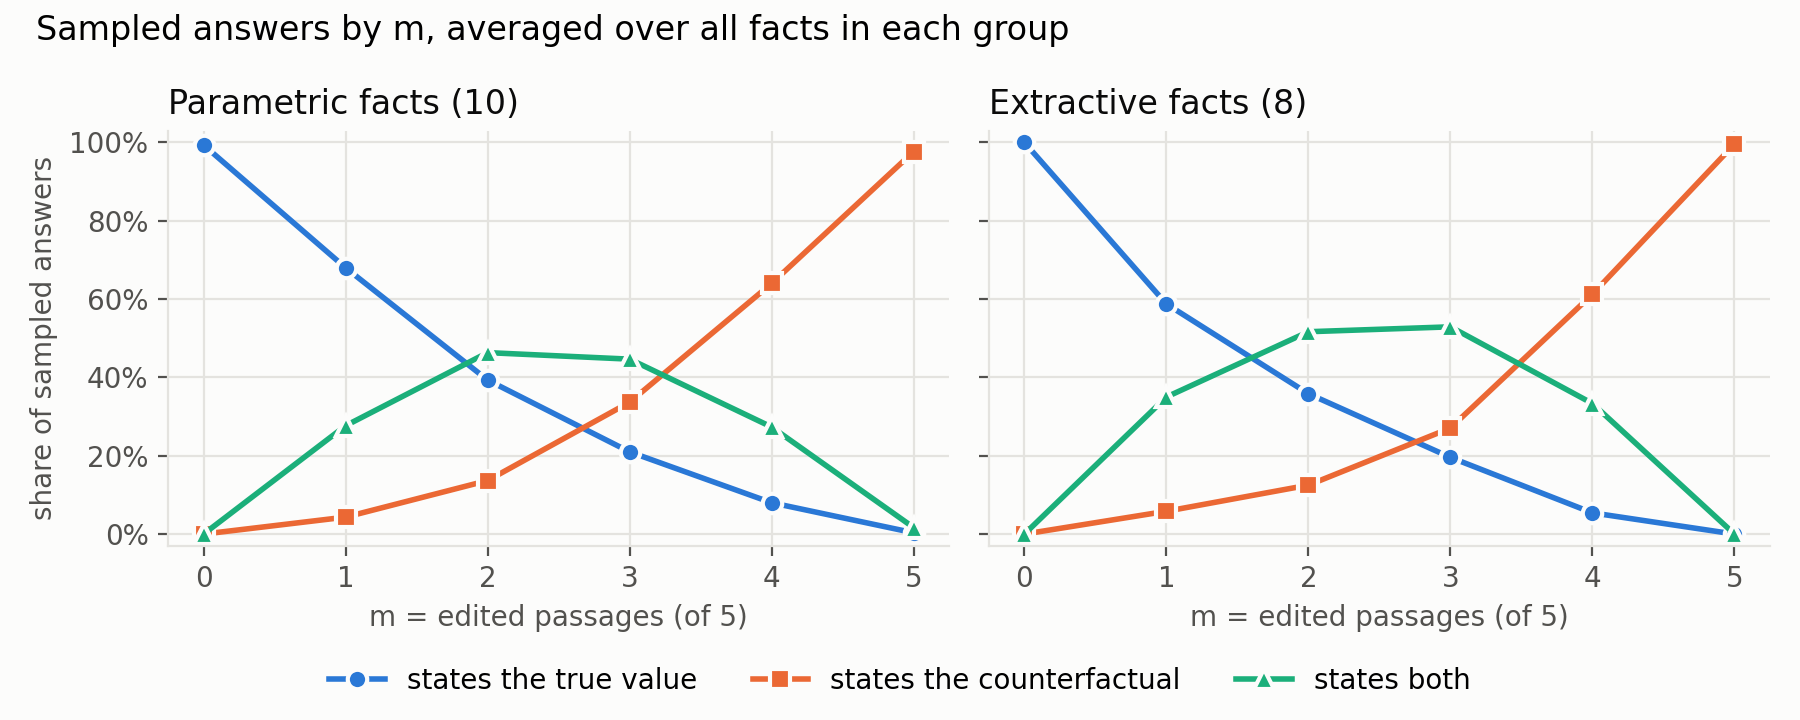
\includegraphics[keepaspectratio,alt={Figure 4: Share of sampled answers that state the true value, the counterfactual value, or both, against the number of edited passages m, averaged over all facts in each group. Left: the 10 parametric facts. Right: the 8 extractive facts.}]{figures/comp345-midterm-fig-dose-by-group.png}}
\caption{Figure 4: Share of sampled answers that
state the true value, the counterfactual value, or
both, against the number of edited passages m,
averaged over all facts in each group. Left: the
10 parametric facts. Right: the 8 extractive
facts.}
\end{figure}

\begin{figure}
\centering
\pandocbounded{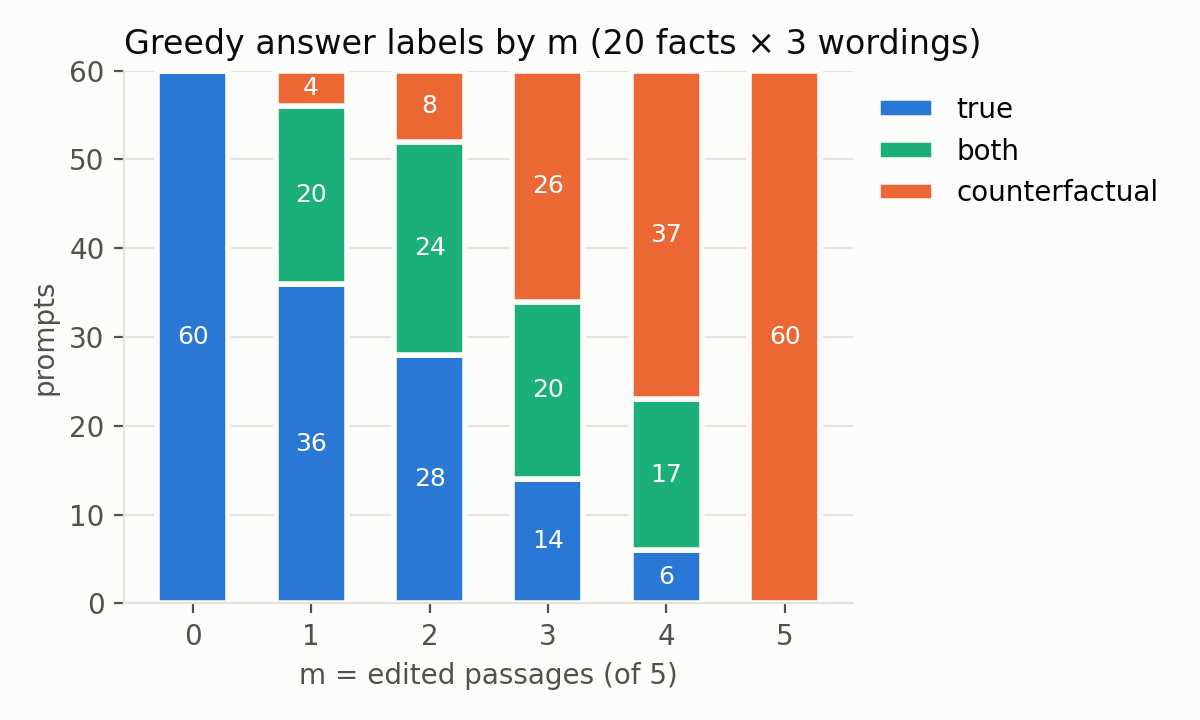
\includegraphics[keepaspectratio,alt={Figure 5: Labels of the greedy answers at each m, for all 20 facts and 3 wordings.}]{figures/comp345-midterm-fig-greedy-labels.png}}
\caption{Figure 5: Labels of the greedy answers at
each m, for all 20 facts and 3 wordings.}
\end{figure}

The flip point is \(m = 2\) for both groups: the
truth-support rate is 57\% (parametric) and 58\%
(extractive) at \(m = 1\), and 47\% and 38\% at
\(m = 2\). The true-answer rate gives the same
flip point. The two groups' curves are nearly
identical (Figure 4). Extractive facts have a
slightly lower true-answer rate at \(m = 1\) (59\%
against 68\%), but with 8 and 10 facts this
difference is within the spread between individual
facts. In this sample, Llama does not keep the
true value for more edited passages on facts it
already knows than on facts it learned only from
the passages, so our second hypothesis is not
supported.

\subsection{7.4 Sigmoid Fits: A Threshold or a
Gradual
Decline?}\label{sigmoid-fits-a-threshold-or-a-gradual-decline}

Our first hypothesis predicts that the true-answer
rate drops sharply over one or two values of
\(m\). The slope \(s\) of each fitted sigmoid
(Section 6.6) measures how sharply the rate falls,
but \(s\) is hard to read on its own, so we
convert \(s\) to a width: the number of edited
passages the fitted curve needs to fall from a
90\% to a 10\% true-answer rate. The width equals
\(2\ln 9 / s \approx 4.4 / s\). A width of 1 or
less means the fact flips within a single added
passage, and a width of 2 or less matches the drop
over one or two values of \(m\) that our first
hypothesis predicts.

Fitted to all 18 RAG prompts of each fact (3
wordings together), as planned in Section 6.6, the
curves look gradual. The median slope is
\(s = 1.5\) for parametric facts and 1.7 for
extractive facts, a median width of 3.0 and 2.5
passages. Only 6 of the 20 facts have a width of 2
or less, and only 3 have a width of 1 or less (the
U.S. corporate tax rate, the year Mexico became
the top U.S. trading partner, and the U.S.
secretary of state).

The pooled fit, however, averages away sudden
drops that appear when each wording is plotted on
its own (Figure 6). Each wording has its own
random order of edited slots, so Passage 1 is
edited at a different \(m\) for each wording, and
each wording drops at a different point. Averaging
three sudden drops at different points produces a
smooth curve. We therefore also fit each of the 60
fact-wording pairs (one fact asked in one wording,
6 prompts each) on its own. The median width is
then 1.4 passages: 38 of the 60 pairs have a width
of 2 or less, and 28 flip within one passage. In
45 of the 60 pairs, a single added passage lowers
the true-answer rate by 50 percentage points or
more. In 30 of the 60 pairs, the largest drop
happens at the step that edits Passage 1, compared
with the 12 we would expect if every passage
mattered equally. For a single question, the
answer therefore usually changes in one step, and
where that step falls depends largely on when
Passage 1 is edited. In the fits by wording, the
extractive facts drop more abruptly (median width
0.7, against 1.6 for parametric facts), but with
these few facts we treat this difference as a
question for the full run.

\begin{figure}
\centering
\pandocbounded{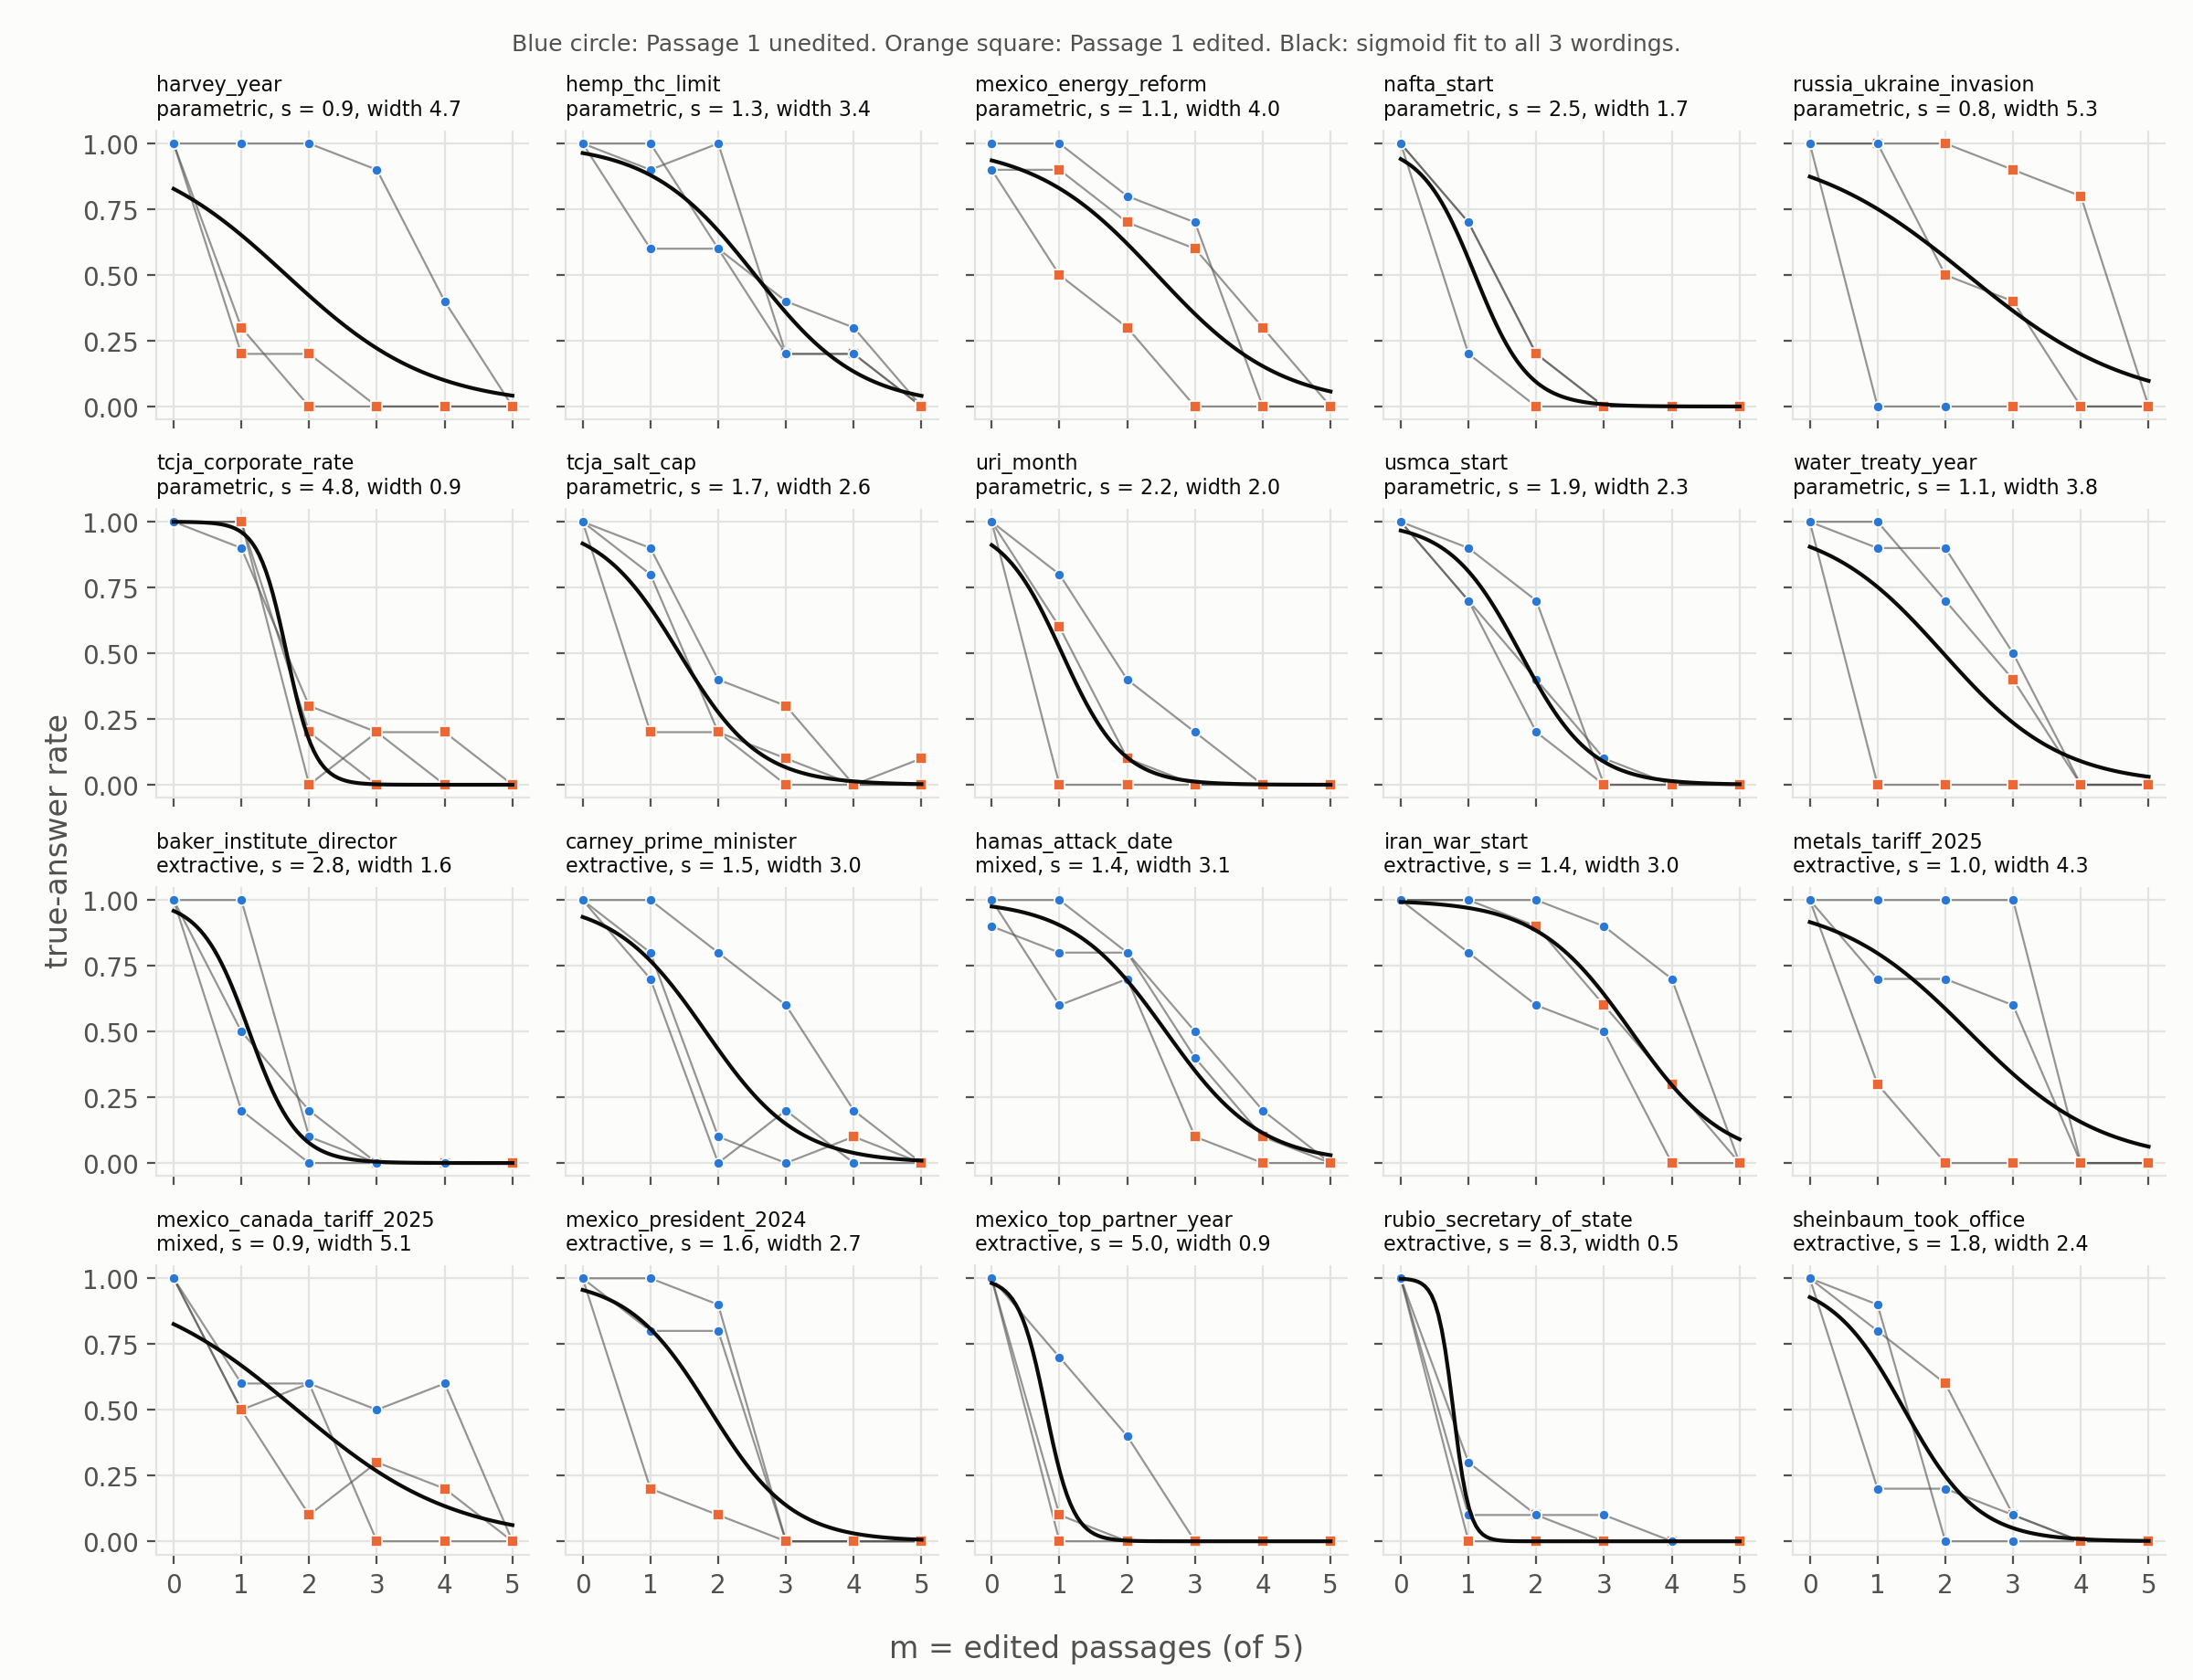
\includegraphics[keepaspectratio,alt={Figure 6: True-answer rate of every fact. Each thin line is one question wording; circles mark prompts where Passage 1 is unedited and squares mark prompts where Passage 1 is edited. The black curve is the sigmoid fitted to all 3 wordings together.}]{figures/comp345-midterm-fig-fact-curves.png}}
\caption{Figure 6: True-answer rate of every fact.
Each thin line is one question wording; circles
mark prompts where Passage 1 is unedited and
squares mark prompts where Passage 1 is edited.
The black curve is the sigmoid fitted to all 3
wordings together.}
\end{figure}

\subsection{7.5 Which Passage
Matters}\label{which-passage-matters}

Which passage is edited changes the answer about
as much as how many passages are edited. Going
from \(m = 0\) to \(m = 5\), the true-answer rate
falls from 99\% to 0\%, so each added edit lowers
the rate by about 20 percentage points on average.
Because the edited slots are nested (Section 6.3),
every step from \(m\) to \(m + 1\) edits exactly
one more passage, so the drop at that step
measures the effect of that one passage. Averaged
over all steps, editing Passage 1 lowers the
true-answer rate by 41 percentage points, Passages
2 and 3 by about 20, and Passages 4 and 5 by about
10 (Figure 7). The gap between editing Passage 1
and editing Passage 5 (about 32 points) is
therefore larger than the average effect of one
more edited passage. Table 3 shows the same
pattern at \(m = 1\): when the one edited passage
is Passage 1, only 36\% of sampled answers state
the true value, but when it is Passage 5, 88\%
still do.

Figure 8 shows the effect of Passage 1 in another
way, by splitting the prompts at each \(m\) by
whether Passage 1 is edited. At every \(m\) from 1
to 4, prompts with an edited Passage 1 have a
lower true-answer rate. With 3 of 5 passages
edited, for instance, Llama gives the true value
in 12 of 24 greedy answers when Passage 1 is
unedited, but in only 2 of 36 when Passage 1 is
edited. The greedy answers also name Passage 1
first far more than any other passage: of the 228
answers that name a passage, 167 start with
Passage 1.

\begin{figure}
\centering
\pandocbounded{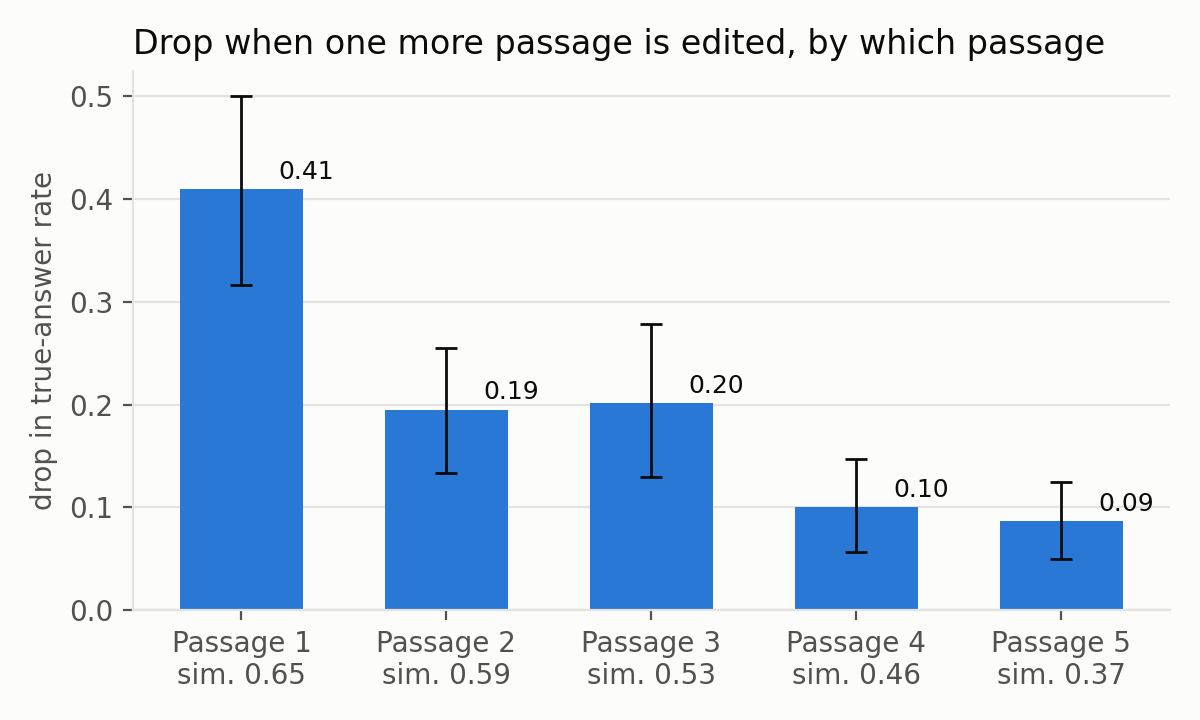
\includegraphics[keepaspectratio,alt={Figure 7: Average drop in the true-answer rate when one more passage is edited, by which passage the step edits (60 steps each). Error bars are 95\% intervals from resampling facts. ``sim.'' is the passage's average retriever similarity to the question.}]{figures/comp345-midterm-fig-step-drops.png}}
\caption{Figure 7: Average drop in the true-answer
rate when one more passage is edited, by which
passage the step edits (60 steps each). Error bars
are 95\% intervals from resampling facts. ``sim.''
is the passage's average retriever similarity to
the question.}
\end{figure}

\begin{figure}
\centering
\pandocbounded{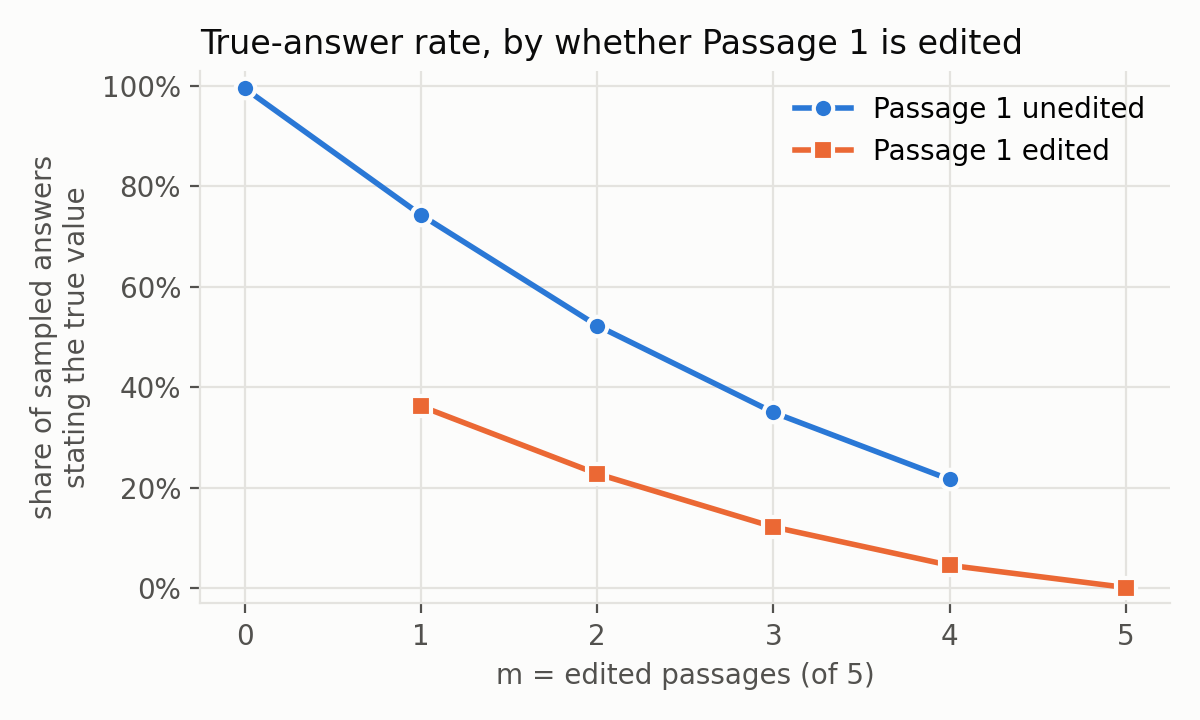
\includegraphics[keepaspectratio,alt={Figure 8: True-answer rate against m, split by whether Passage 1 is edited.}]{figures/comp345-midterm-fig-passage1.png}}
\caption{Figure 8: True-answer rate against m,
split by whether Passage 1 is edited.}
\end{figure}

There are two possible explanations for this
pattern, and our design cannot separate them yet.
The first is position: language models use
information at the start of a long input more than
information in the middle (Liu et al.~2023). The
second is similarity: the retriever places the
passage most similar to the question in slot 1
(average similarity 0.65, against 0.37 for slot
5), so Passage 1 is also the passage that answers
the question most directly. Most wordings fit both
explanations, since the first passage is also the
most similar one. A single wording, however, gives
some evidence for similarity. For ``When did
Russia's full-scale invasion of Ukraine begin?'',
Passage 1 is edited from \(m = 1\), yet 80\% or
more of the sampled answers stay correct up to
\(m = 4\), and the greedy answer cites Passage 3
at every \(m\), including \(m = 0\). Passage 3 is
the only passage that uses the question's own
phrase, ``full-scale invasion,'' and Passage 3 is
not edited until \(m = 5\). Llama appears to
follow the passage whose sentence best matches the
question, and that passage is usually, but not
always, Passage 1. Shuffling the passage order
while keeping the same edits would separate the
two explanations (Section 9).

\emph{Table 3: True-answer rate at m = 1, by which
slot holds the one edited passage.}

{\def\LTcaptype{none} % do not increment counter
\begin{longtable}[]{@{}
  >{\raggedright\arraybackslash}p{(\linewidth - 8\tabcolsep) * \real{0.1967}}
  >{\raggedright\arraybackslash}p{(\linewidth - 8\tabcolsep) * \real{0.1475}}
  >{\raggedright\arraybackslash}p{(\linewidth - 8\tabcolsep) * \real{0.2623}}
  >{\raggedright\arraybackslash}p{(\linewidth - 8\tabcolsep) * \real{0.2295}}
  >{\raggedright\arraybackslash}p{(\linewidth - 8\tabcolsep) * \real{0.1639}}@{}}
\toprule\noalign{}
\begin{minipage}[b]{\linewidth}\raggedright
Edited slot
\end{minipage} &
\begin{minipage}[b]{\linewidth}\raggedright
Prompts
\end{minipage} &
\begin{minipage}[b]{\linewidth}\raggedright
Greedy answers true
\end{minipage} &
\begin{minipage}[b]{\linewidth}\raggedright
True-answer rate
\end{minipage} &
\begin{minipage}[b]{\linewidth}\raggedright
``Both'' rate
\end{minipage} \\
\midrule\noalign{}
\endhead
\bottomrule\noalign{}
\endlastfoot
1 & 16 & 5 & 36\% & 56\% \\
2 & 17 & 10 & 74\% & 22\% \\
3 & 10 & 7 & 59\% & 31\% \\
4 & 8 & 6 & 80\% & 14\% \\
5 & 9 & 8 & 88\% & 12\% \\
\end{longtable}
}

\subsection{7.6 Probe Pilot}\label{probe-pilot}

We trained the 32 layer probes described in
Sections 5.4 and 6.7 on the hidden states of the
360 RAG prompts, using the 5-fold split by fact
from Section 6.7. The target is 1 when the greedy
answer is labelled true (144 of the 360 prompts)
and 0 otherwise, so ``both'' answers count as 0
until they are labelled by hand. Every prompt is
predicted by a probe that never saw its fact. Each
probe is trained with Adam for 500 full-batch
steps (learning rate 0.01, weight decay 0.01).
Before training, each of the 4096 inputs is
rescaled to mean 0 and standard deviation 1 on the
training facts, so that no single input dominates
because of its scale.

The probes do not beat the baseline that sees only
\(m\). The \(m\)-only baseline reaches 80\%
accuracy and an AUC of 0.88 on the held-out facts
(AUC is defined in Section 6.6). The best layer
probes reach an AUC of only 0.59 (layers 23 and
24), and many layers are close to 0.5 (Figure 9).
Within prompts that share the same \(m\), where
the \(m\)-only baseline is at chance by
construction, the best probes reach 0.62 to 0.63
(layers 3, 23, and 24). With only 20 facts, we do
not treat this as evidence that the hidden states
predict the flip, so the pilot does not support
our third hypothesis yet.

The reason appears to be that the fact itself
dominates the hidden state. At layer 16, where the
average hidden-state vector has length 9.7,
editing all 5 passages moves the final token's
vector by only 0.6 on average, while asking the
same question in another wording moves the vector
by 2.7 and switching to another fact moves the
vector by 4.1. A probe trained on 16 facts
therefore learns mostly what separates those facts
from each other, and that does not carry over to
new facts. As a check that the information is
present at all, we also split the prompts at
random, so that every test fact also appears in
training. We do not use this split for results,
because a probe can then score well by recognizing
facts it has already seen. With this split, the
late-layer probes reach an AUC of 0.88. The hidden
states therefore do carry the outcome, but in a
way that our 16 training facts are too few to
separate from the facts themselves.

The control probe, in contrast, performs well.
Trained on the clean prompts (\(m = 0\)) to
predict whether a fact is parametric or
extractive, the control probe reaches 89\%
accuracy on held-out facts at layer 12, where
always guessing the larger group would give 56\%.
The hidden states therefore separate facts Llama
knows from facts it does not. However, most of our
extractive facts concern events from 2023 onward,
so the control probe may partly be detecting
recent topics rather than the model's knowledge
itself.

\begin{figure}
\centering
\pandocbounded{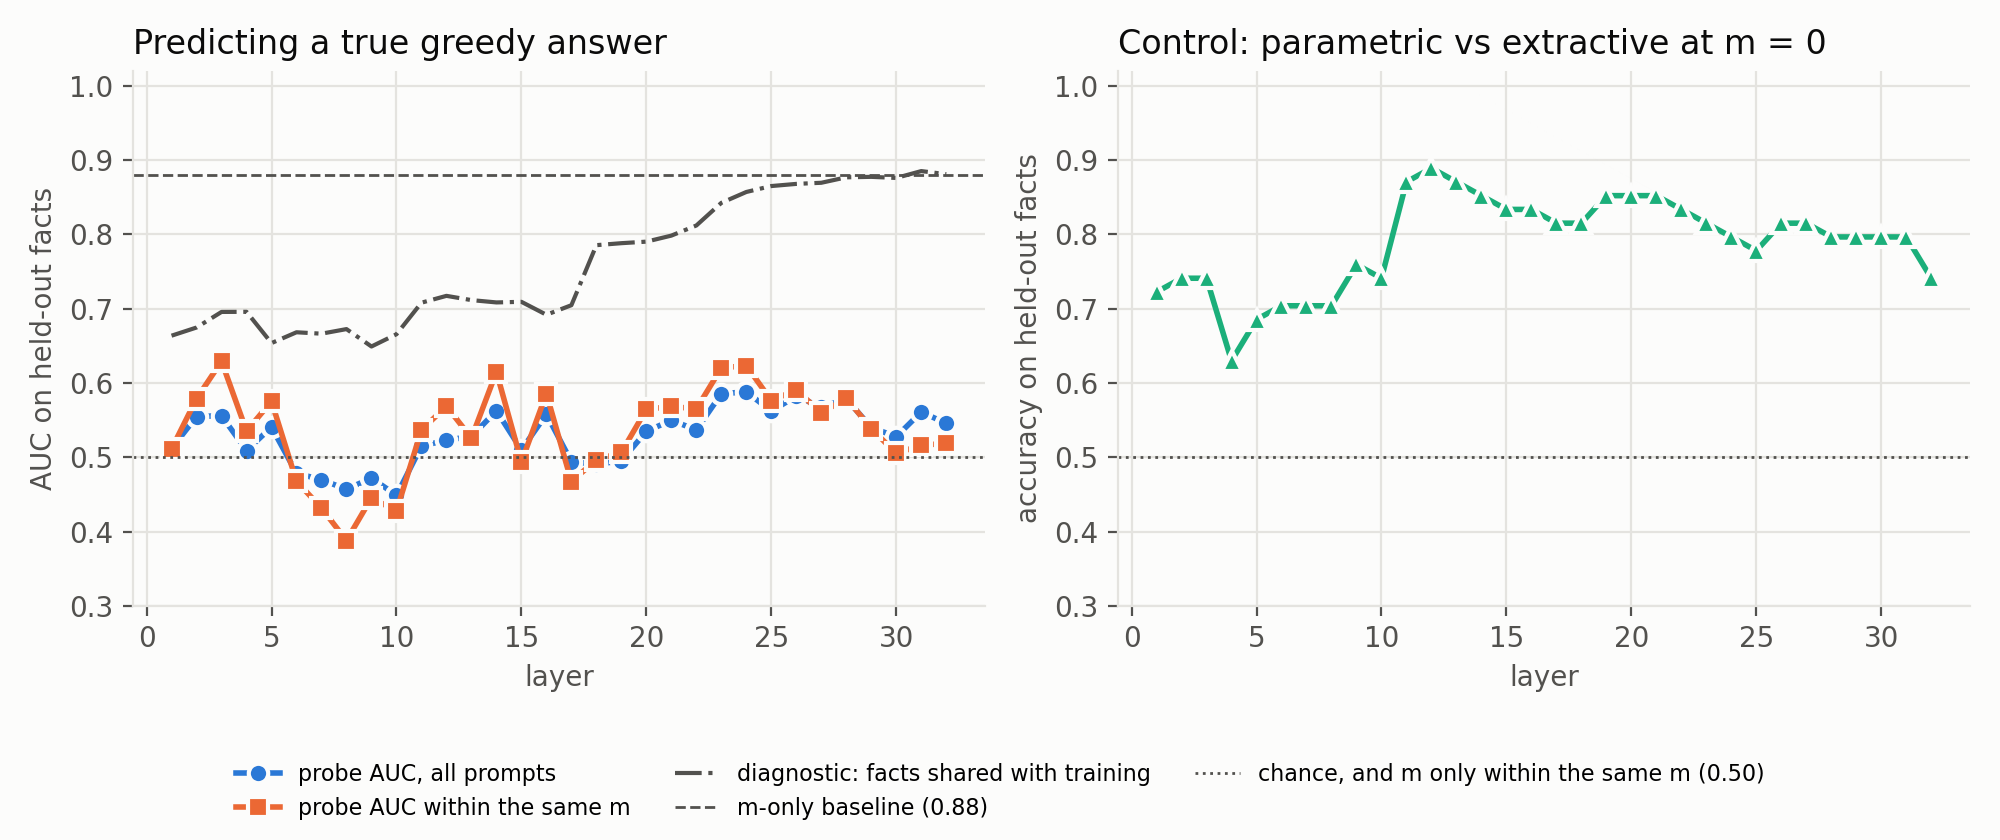
\includegraphics[keepaspectratio,alt={Figure 9: Probe pilot. Left: AUC on held-out facts for predicting a true greedy answer, for all prompts and within prompts that share the same m, with the m-only baseline. The dash-dot line is the diagnostic split that shares facts between training and test. Right: accuracy of the m = 0 control probe that predicts parametric vs extractive.}]{figures/comp345-midterm-fig-probe-layers.png}}
\caption{Figure 9: Probe pilot. Left: AUC on
held-out facts for predicting a true greedy
answer, for all prompts and within prompts that
share the same m, with the m-only baseline. The
dash-dot line is the diagnostic split that shares
facts between training and test. Right: accuracy
of the m = 0 control probe that predicts
parametric vs extractive.}
\end{figure}

\section{8. Failure
Analysis}\label{failure-analysis}

The rates in Section 7 show how often Llama loses
the true value, but not how its answers go wrong.
To see this, we sort every greedy answer that does
not state only the true value (the value in the
unedited passages) into one of four failure types:

\begin{itemize}
\tightlist
\item
  Adopted counterfactual: the answer states the
  counterfactual value.
\item
  Mixed answer: the answer mentions both values
  without picking one.
\item
  Other wrong answer: the answer states a value
  that is neither the true nor the counterfactual
  one.
\item
  Refusal: the model declines to answer.
\end{itemize}

A mixed answer is different from a mixed fact
(Section 4.2). A mixed fact is a fact Llama knows
for only some wordings, while a mixed answer is a
single answer that names both values.

We also note cases where the corpus itself
disagrees about a fact (for example, different
figures from different years or from authors with
different viewpoints), since these natural
conflicts could mix with the counterfactual values
we insert.

\emph{Table 4: Failure types of the greedy
answers, before hand labelling. ``Mixed answer''
is every answer the script labelled ``both''.}

{\def\LTcaptype{none} % do not increment counter
\begin{longtable}[]{@{}
  >{\raggedright\arraybackslash}p{(\linewidth - 8\tabcolsep) * \real{0.1905}}
  >{\raggedright\arraybackslash}p{(\linewidth - 8\tabcolsep) * \real{0.2540}}
  >{\raggedright\arraybackslash}p{(\linewidth - 8\tabcolsep) * \real{0.2063}}
  >{\raggedright\arraybackslash}p{(\linewidth - 8\tabcolsep) * \real{0.2063}}
  >{\raggedright\arraybackslash}p{(\linewidth - 8\tabcolsep) * \real{0.1429}}@{}}
\toprule\noalign{}
\begin{minipage}[b]{\linewidth}\raggedright
\(m\)
\end{minipage} &
\begin{minipage}[b]{\linewidth}\raggedright
Adopted counterfactual
\end{minipage} &
\begin{minipage}[b]{\linewidth}\raggedright
Mixed answer
\end{minipage} &
\begin{minipage}[b]{\linewidth}\raggedright
Other wrong answer
\end{minipage} &
\begin{minipage}[b]{\linewidth}\raggedright
Refusal
\end{minipage} \\
\midrule\noalign{}
\endhead
\bottomrule\noalign{}
\endlastfoot
closed-book & 1 & 0 & 11 & 16 \\
0 & 0 & 0 & 0 & 0 \\
1 & 4 & 20 & 0 & 0 \\
2 & 8 & 24 & 0 & 0 \\
3 & 26 & 20 & 0 & 0 \\
4 & 37 & 17 & 0 & 0 \\
5 & 60 & 0 & 0 & 0 \\
\end{longtable}
}

With passages, Llama's wrong answers fall into
only two types, adopted counterfactual and mixed
answer. With passages, Llama never refused and
never gave a third value. Without passages, the 28
wrong closed-book answers are refusals (16, all
for extractive or mixed facts) or other wrong
answers (11), plus the one counterfactual answer
from Section 7.1.

Mixed answers are the most common failure at
\(m = 1\) and 2 and stay common until \(m = 4\):
81 of the 300 Condition 3 greedy answers state
both values. Many of these answers follow one
passage and then report the other value as a
disagreement. For example, at \(m = 1\) for NAFTA,
the answer gives 1994 ``according to Passage 1''
and then notes that ``Passage 2 mentions that
NAFTA was implemented in January 1996, which is
incorrect.'' The script cannot tell which value
such an answer settles on, so we will label the 81
mixed greedy answers by hand, along with a random
50 of the script's other labels to check the
script's accuracy.

Llama also sometimes names the wrong passage.
Asked who has been Canada's prime minister since
2025 (Mark Carney) at \(m = 4\), one answer says
``According to Passage 3'' but quotes the true
value, which only the unedited Passage 2 states.
The NAFTA answer at \(m = 3\) (Section 7.3) makes
the same kind of mistake. For this reason we use
the passage citations only as a rough signal and
measure position effects from the edited slots
instead (Section 7.5).

While checking facts by hand, we found such
disagreements in the corpus. For instance, some
passages date the Gulf War as ``1990-91'' rather
than giving a single year, and one passage dates
the start of Russia's invasion of Ukraine to
February 22, 2022, two days before the date most
sources give. In both cases, we left the
disagreeing passages out of the fact's 5 passages.
The Gulf War fact uses only passages that give
1991 alone, and the Ukraine fact does not use the
passage that gives February 22. Neither case
affects the results in this report, since the Gulf
War fact is not among the 20 sampled facts and the
Ukraine question asks only for the month.

\section{9. Discussion and
Limitations}\label{discussion-and-limitations}

The overall goal is to find how much wrong context
it takes to override what a model knows, how that
amount changes when the model already knows the
fact, and what the model's hidden states reveal
about its choice between memory and context.

The midterm results partly support our first
hypothesis and do not support our second. For a
single question wording, the true-answer rate
usually falls in one step, as the first hypothesis
predicts, but the step at which it falls depends
largely on when Passage 1 is edited, and averaging
over wordings turns these steps into a gradual
curve. Llama flips at \(m = 2\) whether or not it
knew the fact beforehand, so in this sample its
pretraining does not make it keep the true value
longer. So far, the results suggest that Llama
does not weigh its memory against the passages so
much as weigh the passages against each other.
Llama mostly follows one passage, usually Passage
1, which is both the first passage and the one
most similar to the question, and it reports the
other value as a disagreement. The probe pilot
does not yet support our third hypothesis: trained
on 16 facts, the probes predict the flip on new
facts no better than the \(m\)-only baseline,
because differences between facts dominate the
hidden states. The full set of about 100 facts
gives 80 training facts instead of 16, which is
the first thing to try before changing the probe
design. The control probe does separate known from
unknown facts (89\% accuracy at layer 12), so the
hidden states do encode whether Llama knows a
fact, which is the distinction behind our second
hypothesis.

These results have several limitations. First,
position and similarity are confounded. Passage 1
is always the passage the retriever rates most
similar to the question, so we cannot yet say
whether Llama favors that passage for being first
or for matching the question best. Second, the
sample is small: 20 facts instead of about 100,
with only 8 extractive facts, so the differences
between the two groups are within the spread
between individual facts. Third, the scoring
script matches fixed text patterns, so the 81
greedy answers that state both values still need
hand labels, and until then these answers count as
not true. Fourth, the GPU and the laptop CPU give
slightly different answers to the same prompt, so
every number in this report comes from one GPU
run. Finally, an edit that replaces a year can
also change a range that contains that year. For
instance, for the year Enrique Peña Nieto became
president of Mexico (2012, counterfactual 2013;
not among this report's 20 facts), three passages
give his term as ``2012-2018'', which the edit
turns into a five-year term, ``2013-2018''. Llama
could notice this mismatch, which may make some
edited passages easier to reject than others.
Before the full run, we will search the edited
passages for ranges like this one and replace any
affected passage with one that states the year on
its own.

Before the final report, we plan to:

\begin{itemize}
\tightlist
\item
  check more facts by hand, especially extractive
  facts, to reach about 100;
\item
  label the mixed answers by hand and check a
  random 50 of the script's labels;
\item
  run the full experiment (1,800 RAG examples) on
  the GPU;
\item
  retrain the probes on the full set, which gives
  about 80 training facts instead of 16;
\item
  add a control that shuffles the passage order
  while keeping the same edits, to separate the
  effect of position from the effect of
  similarity;
\item
  run Condition 4 (corpus-level edits) if time
  permits.
\end{itemize}

\section{References}\label{references}

Cuconasu, F., Trappolini, G., Siciliano, F.,
Filice, S., Campagnano, C., Maarek, Y.,
Tonellotto, N., and Silvestri, F. (2024). The
Power of Noise: Redefining Retrieval for RAG
Systems. \emph{ACM SIGIR Conference on Research
and Development in Information Retrieval (SIGIR)}.
arXiv:2401.14887.

Egan, J., Robertson, C. T., Ross Arguedas, A.,
Newman, N., Nielsen, R. K., Mukherjee, M., and
Fletcher, R. (2026). \emph{Reuters Institute
Digital News Report 2026}. Reuters Institute for
the Study of Journalism.
doi:10.60625/risj-4vgf-s811.

Lewis, P., Perez, E., Piktus, A., Petroni, F.,
Karpukhin, V., Goyal, N., Küttler, H., Lewis, M.,
Yih, W., Rocktäschel, T., Riedel, S., and Kiela,
D. (2020). Retrieval-Augmented Generation for
Knowledge-Intensive NLP Tasks. \emph{Advances in
Neural Information Processing Systems (NeurIPS)}.
arXiv:2005.11401.

Liu, N. F., Lin, K., Hewitt, J., Paranjape, A.,
Bevilacqua, M., Petroni, F., and Liang, P. (2023).
Lost in the Middle: How Language Models Use Long
Contexts. \emph{Transactions of the Association
for Computational Linguistics} (2024).
arXiv:2307.03172.

Longpre, S., Perisetla, K., Chen, A., Ramesh, N.,
DuBois, C., and Singh, S. (2021). Entity-Based
Knowledge Conflicts in Question Answering.
\emph{Conference on Empirical Methods in Natural
Language Processing (EMNLP)}. arXiv:2109.05052.

Shi, F., Chen, X., Misra, K., Scales, N., Dohan,
D., Chi, E., Schärli, N., and Zhou, D. (2023).
Large Language Models Can Be Easily Distracted by
Irrelevant Context. \emph{International Conference
on Machine Learning (ICML)}. arXiv:2302.00093.

Wu, K., Wu, E., and Zou, J. (2024). ClashEval:
Quantifying the Tug-of-War between an LLM's
Internal Prior and External Evidence.
\emph{NeurIPS 2024 Datasets and Benchmarks Track}.
arXiv:2404.10198.

Xie, J., Zhang, K., Chen, J., Lou, R., and Su, Y.
(2024). Adaptive Chameleon or Stubborn Sloth:
Revealing the Behavior of Large Language Models in
Knowledge Conflicts. \emph{International
Conference on Learning Representations (ICLR)}.
arXiv:2305.13300.

Zhao, Y., Du, X., Hong, G., Gema, A. P., Devoto,
A., Wang, H., He, X., Wong, K.-F., and Minervini,
P. (2024). Analysing the Residual Stream of
Language Models Under Knowledge Conflicts.
\emph{NeurIPS 2024 Workshop on Foundation Model
Interventions}. arXiv:2410.16090.

\end{document}
